\documentclass[10pt,conference]{IEEEtran}
% \IEEEoverridecommandlockouts
% The preceding line is only needed to identify funding in the first footnote. If that is unneeded, please comment it out.
\usepackage{cite}
\usepackage{amsmath,amssymb,amsfonts}
\usepackage{algorithmic}
\usepackage{graphicx}
\usepackage{textcomp}
\usepackage{xcolor}
\usepackage[hidelinks]{hyperref}
\usepackage{listings}
\usepackage{multirow}
\usepackage{booktabs}
\usepackage{graphics}
\usepackage[absolute,overlay]{textpos}


\lstset{
	basicstyle=\ttfamily\small,
	columns=fullflexible,
	showstringspaces=false,
	commentstyle=\color{gray}\upshape,
% 	numbers=left,                    
% 	numbersep=5pt,                  
	showspaces=false,                
	showstringspaces=false,
	showtabs=false,                  
	tabsize=1
}
\def\BibTeX{{\rm B\kern-.05em{\sc i\kern-.025em b}\kern-.08em
    T\kern-.1667em\lower.7ex\hbox{E}\kern-.125emX}}
    
\makeatletter
 \newcommand{\linebreakand}{%
  \end{@IEEEauthorhalign}
  \hfill\mbox{}\par
  \mbox{}\hfill\begin{@IEEEauthorhalign}
} 

\makeatother



\begin{document}

%\title{GPTShare: How developers learn from ChatGPT in GitHub and Hacker News}
\title{DevGPT:\\Studying Developer-ChatGPT Conversations}

\author{
\IEEEauthorblockN{Tao Xiao}
\IEEEauthorblockA{
\textit{Nara Institute of Science and Technology}\\
Nara, Japan\\
tao.xiao.ts2@is.naist.jp}
\and
\IEEEauthorblockN{Christoph Treude}
\IEEEauthorblockA{
\textit{The University of Melbourne}\\
Melbourne, Australia \\
christoph.treude@unimelb.edu.au}
\and
\linebreakand
\IEEEauthorblockN{Hideaki Hata}
\IEEEauthorblockA{
\textit{Shinshu University}\\
Nagano, Japan \\
hata@shinshu-u.ac.jp}
\and
\IEEEauthorblockN{Kenichi Matsumoto}
\IEEEauthorblockA{
\textit{Nara Institute of Science and Technology}\\
Nara, Japan\\
matumoto@is.naist.jp}
}

% \date{Author pre-print copy.}

\maketitle
\begin{textblock*}{\textwidth}(0.5in,0.5in)  % {block width} (coords)
    \centering \texttt{MSR 2024 Mining Challenge Proposal preprint}
\end{textblock*}
\section{Title of data set}
%GPTShare
\begin{center}
DevGPT
\end{center}


\section{High-level overview}
The emergence of large language models (LLMs) such as ChatGPT has disrupted the landscape of software development. Many studies are investigating the quality of responses generated by ChatGPT, the efficacy of various prompting techniques, and its comparative performance in programming contests, to name a few examples. Yet, we know very little about how ChatGPT is actually used by software developers. What questions do developers present to ChatGPT? What are the dynamics of these interactions? What is the backdrop against which these conversations are held, and how do the conversations feedback into the artifacts of their work? To close this gap, we introduce DevGPT, a curated dataset which encompasses 17,913 prompts and ChatGPT's responses including 11,751 code snippets, coupled with the corresponding software development artifacts---ranging from source code, commits, issues, pull requests, to discussions and Hacker News threads---to enable the analysis of the context and implications of these developer interactions with ChatGPT.

%The trend of Large Language Models (LLMs) started in the developers' society before the world. The GitHub Copilot,\footnote{\url{https://github.com/features/copilot}} which is an extension for the Visual Studio Code development environment, breaks the traditional copy-paste development into code generation from prompt-based models. Although such tools cannot substitute for pair programming, they increase the productivity of software development~\cite{imai2022github}. After one year, the popular LLM chatbot, ChatGPT, has born to make the name `LLM' known worldwide.
%``In 20 years following the internet space, we cannot recall a faster ramp in a consumer internet app,'' USB's analysts wrote in the study.

To create DevGPT, we leveraged a feature introduced by OpenAI in late May 2023, which allows users to share their interactions with ChatGPT through dedicated links.\footnote{\url{https://help.openai.com/en/articles/7925741-chatgpt-shared-links-faq}} We collected all such links shared on GitHub and Hacker News at six specific points in time: July 27, 2023, August 3, 2023, August 10, 2023, August 17, 2023, August 24, 2023, and August 31, 2023. If users chose to delete or deactivate their shared conversations in the intervening periods, we ensured data consistency by accessing the original shared link across all these snapshots.

%OpenAI enables users to share their conversations through the links.\footnote{\url{https://help.openai.com/en/articles/7925741-chatgpt-shared-links-faq}} We built GPTShare to analyze the different usage between GitHub and HackerNews. GPTShare contains three snapshots from July 27, 2023, August 3, 2023, and August 10, 2023. If users delete or inactivate the shared conversations, we obtain the data from the same shared link in all snapshots.
% We then show different data extraction processes in the following:

% \textbf{GitHub GraphQL\footnote{\url{https://docs.github.com/en/graphql}} and REST}:\footnote{\url{https://docs.github.com/en/rest?apiVersion=2022-11-28}} We performed a search function with the keyword ``https://chat.openai.com/share/'' in the GitHub GraphQL API to identify mentions of shared links in issues, pull requests, and discussions from GitHub. Since this function did not support searching special characters (e.g., `/' and `:'), we then identified the exact mentions of shared ChatGPT links by the regular expression:
% \begin{lstlisting}[breaklines=true]
% https:\/\/chat\.openai\.com\/share\/[a-zA-Z0-9-]{36}
% \end{lstlisting}
% For the GitHub REST API, we performed the same keyword and regular expression to obtain the references of shared ChatGPT links in commits and code files from GitHub. 
% Moreover, we applied additional filters (e.g., creation time) in order to work around GitHub’s limit on the search function, since it only supports a maximum of thousand results per call.

% \textbf{HackerNews}: Similar to the GitHub search function, HackerNews also provides an endpoint ( \textit{http://hn.algolia.com/api/v1/search?query=...}) to obtain references of shared ChatGPT links in posts from HackerNews. The same regular expression was applied to further identify whether mentioned links are shared ChatGPT links.

% \textbf{Shared ChatGPT conversations}: After obtaining shared ChatGPT links from different sources, we fetched the web page of the shared conversation from ChatGPT. Since users could delete or inactivate the shared conversations, we fetched all data once a week (three snapshots in total from July 27, 2023, August 3, 2023, and August
% 10, 2023). If the response status is other than \textit{200}, we obtain the data from the same shared link in all snapshots.

\begin{table*}[t]
    \centering
    \caption{Summary Statistics of the snapshot 20230831}
    \label{tab:summary}
    \resizebox{.9\textwidth}{!}{
    \begin{tabular}{lrlrrrrr}
    \toprule
    \textbf{Sources} &  \textbf{\# } &  \textbf{Mentioned in} &  \multicolumn{3}{c}{\textbf{Shared ChatGPT Links}} & \multicolumn{2}{c}{\textbf{ChatGPT Conversations}} \\
    & & & \# Shared Links & \# Accessible Links & \# Conversations with Code & \# Prompts & \# Code Snippets 
    \\
    \midrule
    \multirow{1}{*}{\textbf{GitHub Code File}} & \multirow{1}{*}{970} & Code  & 1386 & 1306 & 577 & 12320 & 7190 \\
    \midrule
    \multirow{1}{*}{\textbf{GitHub Commit}} & \multirow{1}{*}{481} & Message  & 481 & 477 & 470 & 1387 & 1569 \\
    \midrule
    \multirow{3}{*}{\textbf{GitHub Issue}} & \multirow{3}{*}{353}
    &   Comment & 264 & 243 & 160 & 844 & 739\\
    & &  Description & 150 & 138 & 98 & 854 & 757 \\
    & & Title & 3 & 3 & 3 & 49 & 77 \\
    \midrule
    \multirow{3}{*}{\textbf{Hacker News}} & \multirow{3}{*}{195} & Comment  & 274 & 240 & 50 & 837 & 163 \\
    & & Attached URL & 44 & 39 & 3 & 380 & 65 \\
    & & Story & 17 & 14 & 4 & 57 & 66 \\
    \midrule
    \multirow{3}{*}{\textbf{GitHub Pull Request}} & \multirow{3}{*}{193} & Description & 82 & 81 & 57 & 494 & 428\\
    & & Review Thread & 74 & 67 & 48 & 154 & 146 \\
    & & Comment & 65 & 60 & 35 & 351 & 397 \\
    \midrule
    \multirow{3}{*}{\textbf{GitHub Discussion}} & \multirow{3}{*}{45} & Comment & 25 & 22 & 11 & 72 & 37 \\
    & & Description & 20 & 19 & 12 & 89 & 94 \\
    & & Reply & 6 & 5 & 3 & 25 & 23 \\
    \bottomrule
    \end{tabular}}
    
\end{table*}
% 747 + 179 + 235 + 147 + 138 + 32
% 1050 + 179 + 171 + 102 + 3 + 65 +54 +54+168+34 +11+19+16+3

%Table~\ref{tab:summary} provides summary statistics of the DevGPT data set. This data set contains 2,891 shared ChatGPT links from 2,237 GitHub or Hacker News sources with 17,913 prompts/answers, including 11,751 code snippets. The top three common types of code snippets are Python (1,735), JavaScript (1,530), and Bash (1,435). From 2,891 shared ChatGPT links, 2,137 links are accessible, and 1,185 of these links contain at least one code snippet in answers from ChatGPT. We also found that 461 shared ChatGPT links are mentioned in different sources. In other words, we identified 2,345 unique shared ChatGPT links in DevGPT. Figure~\ref{fig:exm} presents the example of mentioning ChatGPT shared conversation in the GitHub Pull Request, where important attributes are highlighted.

Table~\ref{tab:summary} provides an overview of the snapshot 20230831. Comprising 2,891 shared ChatGPT links sourced from 2,237 GitHub or Hacker News references, the dataset contains a total of 17,913 prompts/answers. This includes 11,751 code snippets, with Python (1,735), JavaScript (1,530), and Bash (1,435) as the top three programming languages. 546 of these links are referenced across multiple sources, resulting in a unique count of 2,345 individual ChatGPT shared links within DevGPT. We will periodically expand the DevGPT dataset until its official release for the MSR mining challenge. Figure~\ref{fig:exm} shows an instance of a ChatGPT conversation from the dataset, together with the pull request it was related to and how the code was updated after the ChatGPT conversation.

\begin{figure*}[h]
\caption{Example of a ChatGPT conversation in the context of a GitHub pull request}
\label{fig:exm}
\centering
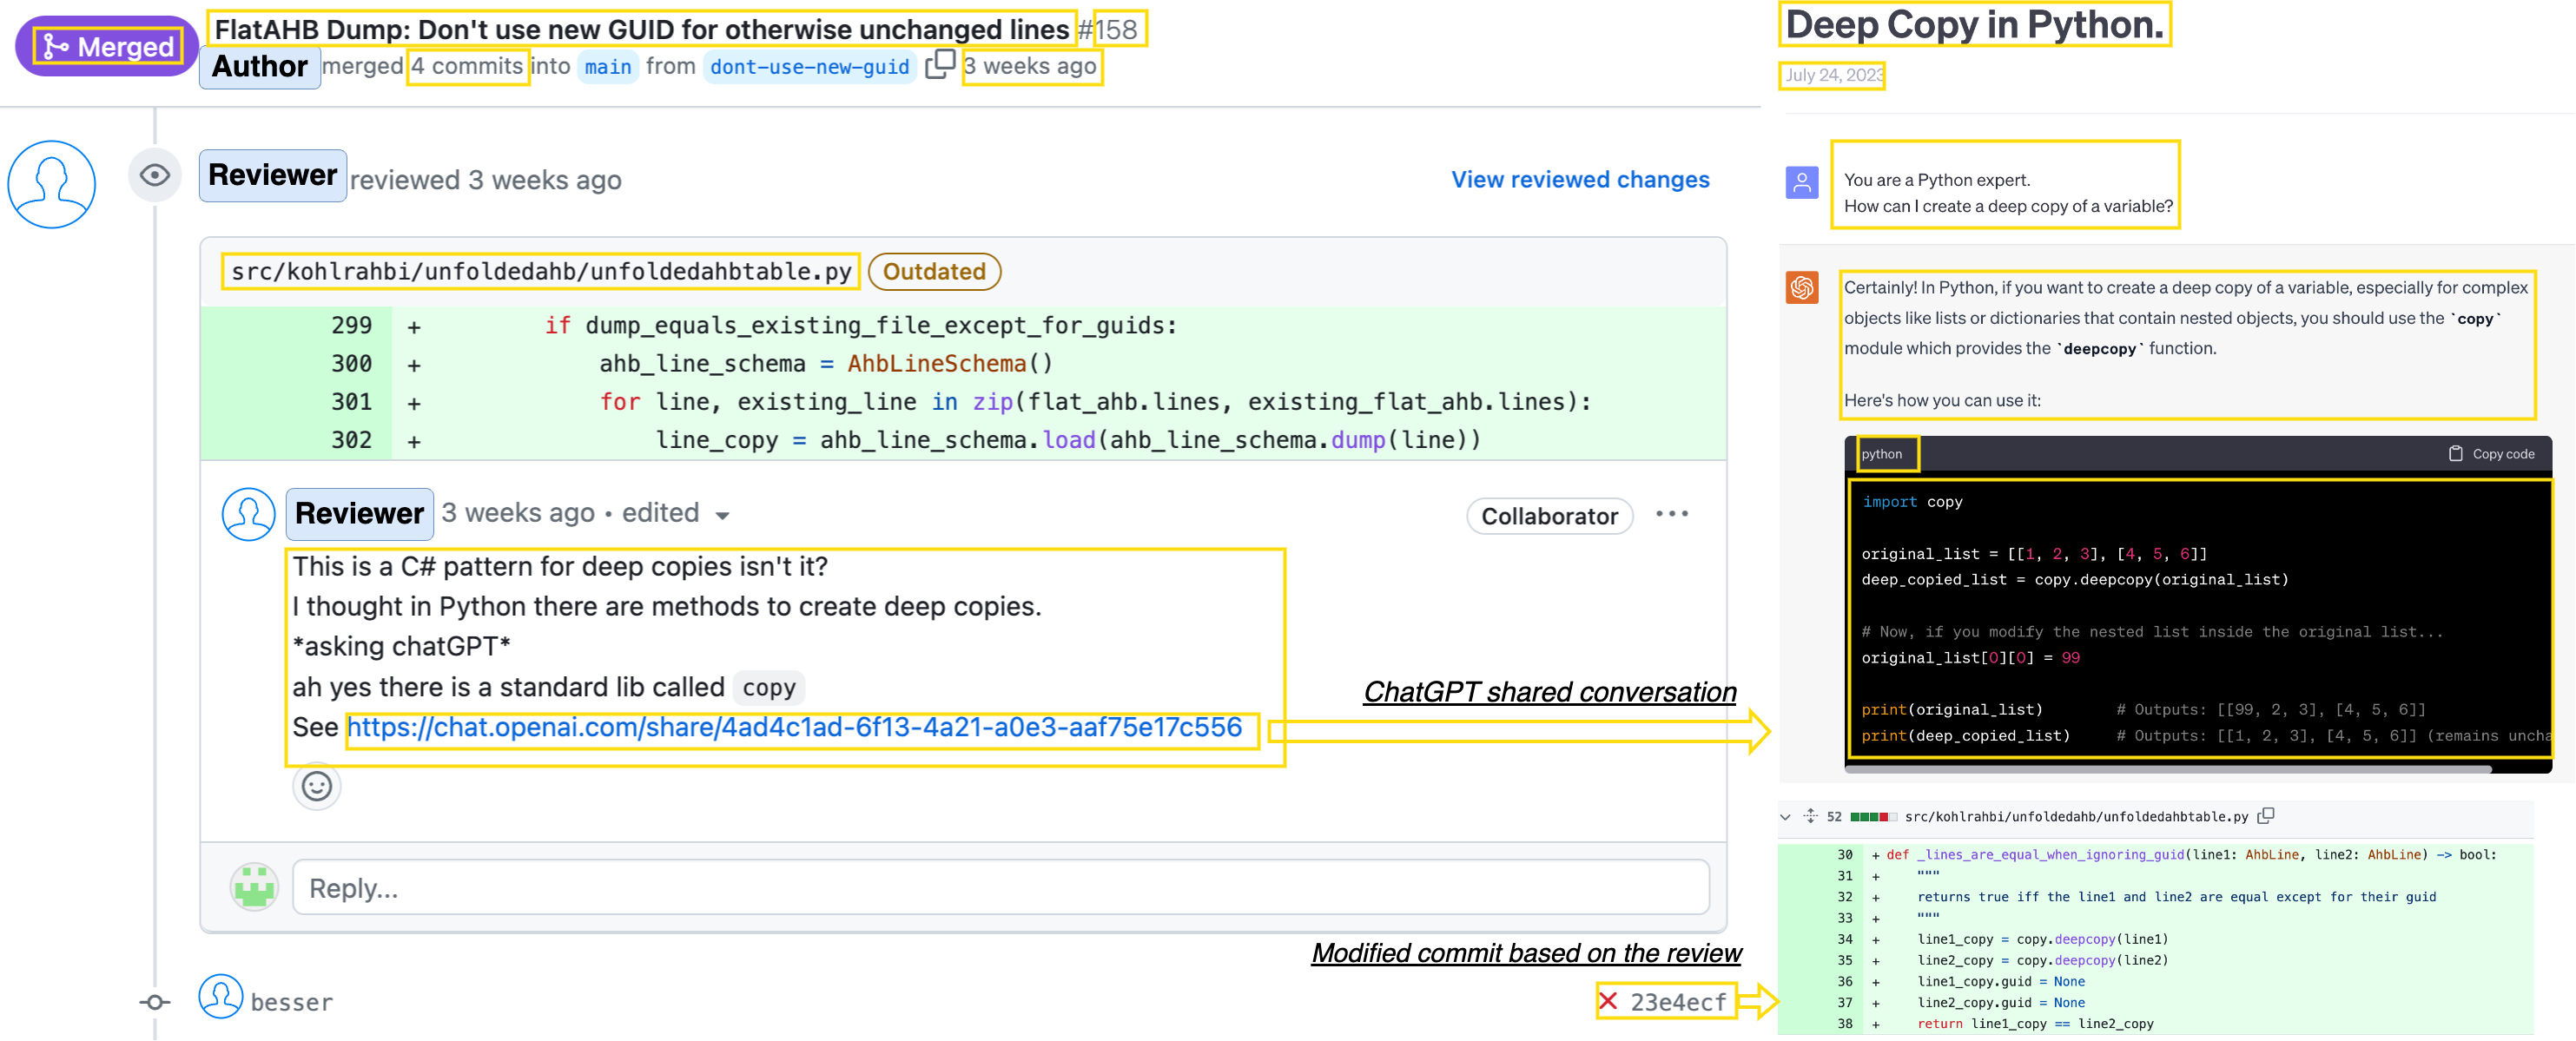
\includegraphics[width=\textwidth]{example.png}
\end{figure*}

\section{Internal structure}
%The data is provided as a set of JSON files from six sources in Table~\ref{tab:summary}. Each source will provide different metadata in the JSON file according to different APIs and needs for analyses. Other than the metadata, the common attribute is a list of shared ChatGPT links in each case of sources. For shared ChatGPT link, it consists of the URL to the shared ChatGPT conversation, the status codes of the HTTP response, the date when we accessed this URL, and the content in this HTML response. Additionally, each conversation contains a list of prompts/answers with code snippets. We obtained the date of the conversation, the number of prompts/answers, the tokens of these prompts/answers, and the model used in this conversation. We also put the attributes of where it has been mentioned, i.g., URL to where it was mentioned, what kind of property mentioned it (e.g., comment), who mentioned it, and the context that mentioned it. The detailed data structure could be found in the replication package. We provide a CSV file including all shared ChatGPT links that we collected from GitHub and Hacker News.

The dataset consists of a collection of JSON files collected from the six sources detailed in Table~\ref{tab:summary}. For each source, we provide distinct metadata in the JSON file to enable source-specific analysis. Apart from the source-specific metadata, every JSON contains a consistent attribute: a list of shared ChatGPT links. Each shared link includes the URL to the ChatGPT conversation, the associated HTTP response status codes, the access date of the URL, and the content within the HTML response. Additionally, each conversation contains a list of prompts/answers, inclusive of any code snippets. We provide details including the date of the conversation, the count of prompts/answers, their token information, and the model version involved in the chat. Attributes detailing where the conversation was referenced are also included---such as the referencing URL, the nature of the mention (e.g., a comment), the individual who mentioned it, and the context in which it was cited. A comprehensive breakdown of the data structure is available at \url{https://github.com/NAIST-SE/DevGPT}. Additionally, we provide a CSV file cataloging all shared ChatGPT links gathered from GitHub and Hacker News.

\section{How to access}
%The DevGPT data set can be downloaded from Zenodo (see Section~\ref{sec:link}). Any JSON library can be used to parse this JSON data. We also provide the content of the HTTP response to shared ChatGPT links, thereby any HTML parser can analyze the content in the conversation. Moreover, we provide types of code snippets in this data set, so that researchers could use the corresponding compilers to execute code. We encourage researchers to register for an account with the respective tools (ChatGPT, GitHub, and Hacker News). Lastly, no credentials are required to access the data.

The DevGPT dataset is available for download on Zenodo, see Section~\ref{sec:link}. It is formatted in JSON, making it easily parsable with any standard JSON library. Additionally, we include the HTTP response, which can be analyzed using any HTML parser. The dataset also categorizes code snippets by type, enabling researchers to use corresponding compilers for execution. No credentials are needed to access the dataset.

\section{Potential research questions}
The following provides a sample list of research questions that can be answered with the DevGPT dataset:
\begin{enumerate}
    \item What types of issues (bugs, feature requests, theoretical questions, etc.) do developers most commonly present to ChatGPT?
    \item Can we identify patterns in the prompts developers use when interacting with ChatGPT, and do these patterns correlate with the success of issue resolution?
    \item What is the typical structure of conversations between developers and ChatGPT? How many turns does it take on average to reach a conclusion?
    \item In instances where developers have incorporated the code provided by ChatGPT into their projects, to what extent do they modify this code prior to use, and what are the common types of modifications made?
    \item How does the code generated by ChatGPT for a given query compare to code that could be found for the same query on the internet (e.g., on Stack Overflow)?
    \item What types of quality issues (for example, as identified by linters) are common in the code generated by ChatGPT?
    \item How accurately can we predict the length of a conversation with ChatGPT based on the initial prompt and context provided?
    \item Can we reliably predict whether a developer's issue will be resolved based on the initial conversation with ChatGPT?
    \item If developers were to rerun their prompts with ChatGPT now and/or with different settings, would they obtain the same results?
\end{enumerate}

\section{Links}
\label{sec:link}
\url{https://github.com/NAIST-SE/DevGPT} and
\url{https://doi.org/10.5281/zenodo.8304091}


%\bibliographystyle{IEEEtran}
%\bibliography{main}


\end{document}
